% !TeX program = pdflatex
\documentclass[11pt]{article}

% --- arXiv-compatible packages ---
\usepackage[utf8]{inputenc}
\usepackage[T1]{fontenc}
\usepackage[brazilian]{babel}
\usepackage{microtype}
\usepackage{amsmath,amssymb,amsfonts}
\usepackage{graphicx}
\usepackage{booktabs}
\usepackage{multirow}
\usepackage{hyperref}
\usepackage{xcolor}
\usepackage{enumitem}
\usepackage[margin=1in]{geometry}
\usepackage{caption}
\usepackage{subcaption}
\usepackage{natbib}
\bibliographystyle{plainnat}

\hypersetup{
    colorlinks=true,
    linkcolor=blue!70!black,
    citecolor=blue!70!black,
    urlcolor=blue!70!black
}

% --- Custom commands ---
\newcommand{\talkex}{\textsc{TalkEx}}
\newcommand{\macrof}{Macro-F1}
\newcommand{\pp}{\,pp}

\title{%
\talkex{}: Uma Arquitetura Híbrida Cascateada para\\
Classificação de Intenções em Conversas\\[6pt]
\large Combinando BM25, Embeddings Congelados e Regras Determinísticas\\
sobre Conversas Multi-Turno de Atendimento ao Cliente em PT-BR%
}

\author{%
Paulo Henrique Vieira Nascimento\thanks{Mestrando, MIT Media Lab (Conversation Intelligence Group). Correspondência: \texttt{paulohenriquevn@gmail.com}}
}

\date{Março 2026}

\begin{document}
\maketitle

% ============================================================================
% RESUMO
% ============================================================================
\begin{abstract}
Apresentamos o \talkex{}, um pipeline modular de PLN para classificação de intenções em conversas de atendimento ao cliente em português brasileiro. O \talkex{} combina três paradigmas tipicamente estudados de forma isolada: recuperação lexical BM25, embeddings multilíngues congelados de sentenças (\texttt{paraphrase-multilingual-MiniLM-L12-v2}, 384 dimensões) e um motor de regras semânticas determinísticas compilado a partir de uma linguagem de domínio específico (DSL) em árvores sintáticas abstratas tipadas (ASTs). Avaliamos quatro hipóteses sobre um corpus pós-auditoria de 2.122 conversas em PT-BR abrangendo 8 classes de intenção, utilizando 5 sementes aleatórias e testes de Wilcoxon. \textbf{H1} (recuperação híbrida): confirmada --- Hybrid-LINEAR atinge MRR\,=\,0,853 vs.\ BM25 0,835 ($p$\,=\,0,017, $r$\,=\,0,29). \textbf{H2} (features combinadas): confirmada --- lexical+embedding LightGBM atinge \macrof{}\,=\,0,722 vs.\ lexical-only 0,334 ($p$\,$<$\,$10^{-35}$, $r$\,=\,0,84). \textbf{H3} (integração de regras): inconclusiva --- regras-como-features resultam em \macrof{}\,=\,0,740 vs.\ ML-only 0,722 ($+1{,}8\pp$, $p$\,=\,0,131), enquanto regras-como-override \emph{degradam} o desempenho ($p$\,$<$\,$10^{-4}$). \textbf{H4} (inferência cascateada): refutada --- uma inversão estrutural de custos torna a cascata mais cara que o pipeline uniforme. Um estudo de ablação quantifica as contribuições dos componentes: embeddings $+33{,}0\pp$, lexical $+2{,}9\pp$, regras $+1{,}8\pp$, estrutural $+1{,}3\pp$. A classificação LightGBM treina em $\sim$6 segundos em CPU sem fine-tuning do codificador; a geração de embeddings utiliza aceleração GPU no Google Colab (Tesla T4), demonstrando que classificação competitiva de intenções é alcançável em infraestrutura de nuvem gratuita.

\medskip
\noindent\textbf{Palavras-chave:} recuperação híbrida, classificação de intenções, BM25, embeddings de sentenças, motor de regras, português brasileiro, atendimento ao cliente, inteligência conversacional
\end{abstract}

% ============================================================================
% 1. INTRODUÇÃO
% ============================================================================
\section{Introdução}
\label{sec:intro}

Operações de atendimento ao cliente no Brasil geram milhões de conversas por mês através de canais de voz, chat, e-mail e redes sociais. Estimativas da indústria indicam que menos de 5\% dessas conversas recebem tratamento analítico além dos códigos de disposição manuais dos agentes --- uma categorização amplamente reconhecida como inconsistente e grosseira. Os 95\% restantes persistem como dados não estruturados, inacessíveis para busca, classificação ou análise de tendências em escala.

Essa lacuna analítica tem consequências concretas: equipes de compliance não conseguem auditar o comportamento dos agentes em escala, sinais de churn que abrangem múltiplos turnos passam despercebidos, e a garantia de qualidade depende de códigos auto-reportados não confiáveis. Sistemas automatizados de inteligência conversacional que classifiquem intenções, recuperem interações similares e produzam evidências auditáveis para cada decisão atenderiam diretamente a essas necessidades operacionais.

Três paradigmas de PLN oferecem capacidades complementares para essa tarefa:

\begin{enumerate}[leftmargin=*,itemsep=2pt]
    \item \textbf{Recuperação lexical} (BM25) destaca-se na correspondência exata de termos --- nomes de produtos, palavras-chave regulatórias, verbos de cancelamento --- mas falha em paráfrases e intenção implícita.
    \item \textbf{Embeddings densos} de codificadores de sentenças pré-treinados capturam similaridade semântica e invariância a paráfrases, mas têm dificuldade com vocabulário específico do domínio e correspondência exata de termos.
    \item \textbf{Regras determinísticas} fornecem precisão controlável e evidência auditável para padrões conhecidos, mas não conseguem generalizar além de sua cobertura lexical.
\end{enumerate}

Esses paradigmas são predominantemente estudados de forma isolada. Trabalhos de recuperação híbrida focam em benchmarks de recuperação de passagens em inglês \citep{formal2021splade,khattab2020colbert,karpukhin2020dense}. Classificação baseada em embeddings tipicamente realiza fine-tuning dos codificadores \citep{tunstall2022setfit,reimers2019sentencebert}. Motores de regras são independentes ou completamente substituídos por sistemas neurais. A integração dos três dentro de um pipeline unificado, avaliado sobre dados conversacionais multi-turno em um idioma diferente do inglês, permanece inexplorada.

O \talkex{} aborda essa lacuna. Propomos uma arquitetura modular cascateada que combina BM25, embeddings multilíngues congelados, classificação supervisionada (LightGBM) e um motor de regras semânticas compilado a partir de uma DSL. Avaliamos quatro hipóteses sobre um corpus de 2.122 registros de atendimento ao cliente em PT-BR com 8 classes de intenção:

\begin{description}[leftmargin=0.5cm,itemsep=2pt]
    \item[H1] Recuperação híbrida (BM25 + ANN) supera a recuperação isolada em MRR.
    \item[H2] Features lexicais + embeddings combinadas superam features apenas lexicais em \macrof{}.
    \item[H3] Regras determinísticas complementam a classificação por ML.
    \item[H4] Inferência cascateada reduz o custo computacional sem perda de qualidade.
\end{description}

Nossas contribuições são: (1) evidência empírica de complementaridade de recuperação híbrida no domínio conversacional em PT-BR; (2) classificação competitiva de intenções (\macrof{}\,=\,0,722) sem fine-tuning, treinando em $\sim$6 segundos no Google Colab; (3) a primeira comparação empírica de três estratégias de integração de regras (features, override, standalone) dentro de um pipeline conversacional unificado; (4) um resultado negativo honesto sobre inferência cascateada, com análise estrutural de por que o modelo de custos falha; e (5) \talkex{}, um framework open-source implementando o pipeline completo com 1.883+ testes automatizados.


% ============================================================================
% 2. TRABALHOS RELACIONADOS
% ============================================================================
\section{Trabalhos Relacionados}
\label{sec:related}

\paragraph{Recuperação Híbrida.} A complementaridade de sinais lexicais e semânticos foi validada em múltiplos benchmarks. O SPLADE \citep{formal2021splade} aprende representações esparsas a partir de cabeçotes MLM; o ColBERT \citep{khattab2020colbert} introduz interação tardia via correspondência no nível de tokens; o DPR \citep{karpukhin2020dense} treina bi-encoders em pares de pergunta-passagem. \citet{rayo2025hybrid} fornecem o precedente metodológico mais próximo, alcançando Recall@10\,=\,0,833 com fusão híbrida BM25 + BGE em textos regulatórios ($\alpha$\,=\,0,65). Porém, seu corpus é de texto regulatório formal em inglês --- estruturalmente diferente de conversas informais multi-turno em PT-BR. \citet{harris2024bm25} demonstram que o BM25 supera modelos semânticos genéricos em documentos médicos estruturados, reforçando o princípio ``sempre avaliar o BM25 primeiro''.

\paragraph{Classificação Baseada em Embeddings.} \citet{reimers2019sentencebert} demonstraram que codificadores de sentenças treinados contrastivamente produzem espaços de similaridade significativos. O SetFit \citep{tunstall2022setfit} alcança classificação competitiva em few-shot usando embeddings de sentenças. O paradigma ``embeddings representam, classificadores decidem'' \citep{anthusai2024embeddings} separa representação de tomada de decisão. A maioria dos trabalhos anteriores realiza fine-tuning nos codificadores; utilizar um codificador multilíngue \emph{congelado} com gradient boosting em PT-BR é, até onde sabemos, inédito.

\paragraph{PLN Baseado em Regras.} O SystemT \citep{chiticariu2013systemT} demonstrou extração baseada em regras em escala industrial. O Snorkel \citep{ratner2017snorkel} utiliza funções de rotulação como supervisão fraca. Motores de produção (Rasa, Dialogflow) suportam regras, mas não as integram como features suaves de ML. A integração suave de regras compiladas via DSL como features do classificador (em vez de overrides rígidos) é uma contribuição original.

\paragraph{Classificação de Intenções Conversacionais.} Benchmarks padrão (CLINC150, BANKING77) são em inglês, turno único e enunciado único. Modelagem multi-turno \citep{zhang2021multi} e classificação baseada em atenção \citep{lyu2025attention} abordam contexto mais rico, mas permanecem focados no inglês. Classificação de intenções conversacionais em PT-BR é virtualmente inexplorada.

\paragraph{PLN em Português.} O BERTimbau \citep{souza2020bertimbau} fornece BERT para PT-BR, mas nenhum dataset público de atendimento ao cliente multi-turno com anotações de intenção existia antes deste trabalho.


% ============================================================================
% 3. ARQUITETURA DO TALKEX
% ============================================================================
\section{Arquitetura do \talkex{}}
\label{sec:architecture}

O \talkex{} implementa um pipeline de PLN multi-estágio com processamento cascateado:

\begin{enumerate}[leftmargin=*,itemsep=2pt]
    \item \textbf{Ingestão e Segmentação de Turnos.} Conversas brutas são parseadas, atribuídas a falantes e segmentadas em turnos usando o \texttt{TurnSegmenter}.
    \item \textbf{Construção de Janelas de Contexto.} O \texttt{SlidingWindowBuilder} gera janelas sobrepostas de 5 turnos (stride 2), capturando dependências multi-turno.
    \item \textbf{Normalização de Texto.} Decomposição Unicode NFD remove diacríticos; case folding garante que ``não'' e ``nao'' correspondam. Crítico para PT-BR.
    \item \textbf{Geração de Embeddings.} \texttt{paraphrase-multilingual-MiniLM-L12-v2} (384 dims, congelado) gera embeddings no nível de turno e janela via mean pooling.
    \item \textbf{Recuperação Híbrida.} BM25 (via \texttt{rank-bm25}) e ANN (via FAISS flat index) produzem listas independentes de top-$K$ candidatos, fundidas via interpolação linear: $S = \alpha \cdot s_{\text{BM25}} + (1-\alpha) \cdot s_{\text{ANN}}$.
    \item \textbf{Classificação.} LightGBM (100 estimadores, 31 folhas) treinado em features concatenadas: TF-IDF (7 dims), scores BM25 (2 dims), metadados estruturais (4 dims), embeddings de 384 dims e flags binárias de ativação de regras (2 dims). Total: 397 features para o pipeline completo.
    \item \textbf{Motor de Regras Semânticas.} Uma DSL é compilada para ASTs tipadas suportando predicados lexicais (\texttt{contains\_any}, \texttt{regex}), predicados semânticos (\texttt{intent\_score}, \texttt{embedding\_similarity}), predicados estruturais (\texttt{speaker}, \texttt{channel}) e predicados contextuais (\texttt{repeated\_in\_window}). Cada execução de regra produz evidência rastreável.
    \item \textbf{Agregação Janela-para-Conversa.} Probabilidades de classe por janela são promediadas; o rótulo final é determinado por argmax sobre a distribuição média.
\end{enumerate}

\noindent\textbf{Axiomas de Design.} \emph{Embeddings representam, classificadores decidem} --- similaridade cosseno nunca é tratada como classificação. \emph{Sempre avaliar o BM25} antes de abordagens semânticas. \emph{LLMs apenas offline} --- modelos leves para inferência online. \emph{Toda predição carrega evidência} --- rótulo, score, confiança, threshold, versão do modelo e evidência textual.


% ============================================================================
% 4. CONFIGURAÇÃO EXPERIMENTAL
% ============================================================================
\section{Configuração Experimental}
\label{sec:setup}

\subsection{Dataset}

Utilizamos o dataset \texttt{RichardSakaguchiMS/brazilian-customer-service-conversations} (HuggingFace, Apache 2.0), expandido com geração sintética controlada (Claude Sonnet, batch offline). Uma auditoria abrangente removeu 135 registros (duplicatas, contaminação few-shot, rótulos ambíguos), consolidando a taxonomia de 9 para 8 classes de intenção ao eliminar \texttt{outros}. A revisão humana confirmou $\geq$96,7\% de acurácia nos rótulos.

\begin{figure}[t]
    \centering
    
\includegraphics[width=\linewidth]{fig_dataset_distribution.pdf}
    \caption{Corpus pós-auditoria: 2.122 conversas em 8 classes de intenção. (a) Distribuição geral das classes mostrando desbalanceamento natural (reclamação 17,3\% a elogio 6,9\%). (b) Splits estratificados treino/validação/teste preservando proporções de classe.}
    \label{fig:dataset}
\end{figure}

O corpus pós-auditoria compreende 2.122 conversas (847 originais + 1.275 sintéticas) com 8 classes de intenção: \textit{cancelamento} (213), \textit{compra} (238), \textit{dúvida\_produto} (340), \textit{dúvida\_serviço} (334), \textit{elogio} (147), \textit{reclamação} (368), \textit{saudação} (172) e \textit{suporte\_técnico} (310). A Figura~\ref{fig:dataset} apresenta a distribuição.

\subsection{Protocolo}

Todos os experimentos utilizam 5 sementes aleatórias [13, 42, 123, 2024, 999] com splits estratificados 70/15/15\% treino/validação/teste no nível da \emph{conversa} (prevenindo vazamento no nível de janela). Resultados são reportados como média $\pm$ desvio padrão entre sementes. Significância estatística é avaliada via testes de Wilcoxon signed-rank ($\alpha$\,=\,0,05) com ICs bootstrap de 95\% (10.000 reamostras). Tamanhos de efeito são reportados como $r = Z/\sqrt{N}$.

\subsection{Métricas}

\textbf{H1:} MRR (primária), Recall@$K$, nDCG@$K$ para $K \in \{5, 10, 20\}$. \textbf{H2/H3:} \macrof{} (primária), F1 por classe, acurácia. \textbf{H4:} Custo por janela (ms), $\Delta$F1, \% resolvido por estágio.

\subsection{Infraestrutura}

Todos os experimentos foram executados no Google Colab com GPU Tesla T4 (15\,GB VRAM). A geração de embeddings utiliza aceleração GPU via PyTorch/CUDA; a classificação LightGBM treina em CPU ($\sim$6 segundos). A suíte completa de experimentos conclui em menos de 1 hora. Software: Python 3.11+, sentence-transformers, scikit-learn, LightGBM, FAISS (cpu), rank-bm25. O código do \talkex{} inclui 1.883+ testes automatizados.


% ============================================================================
% 5. RESULTADOS
% ============================================================================
\section{Resultados}
\label{sec:results}

% --- H1 ---
\subsection{H1: Recuperação Híbrida (Confirmada)}

\begin{figure}[t]
    \centering
    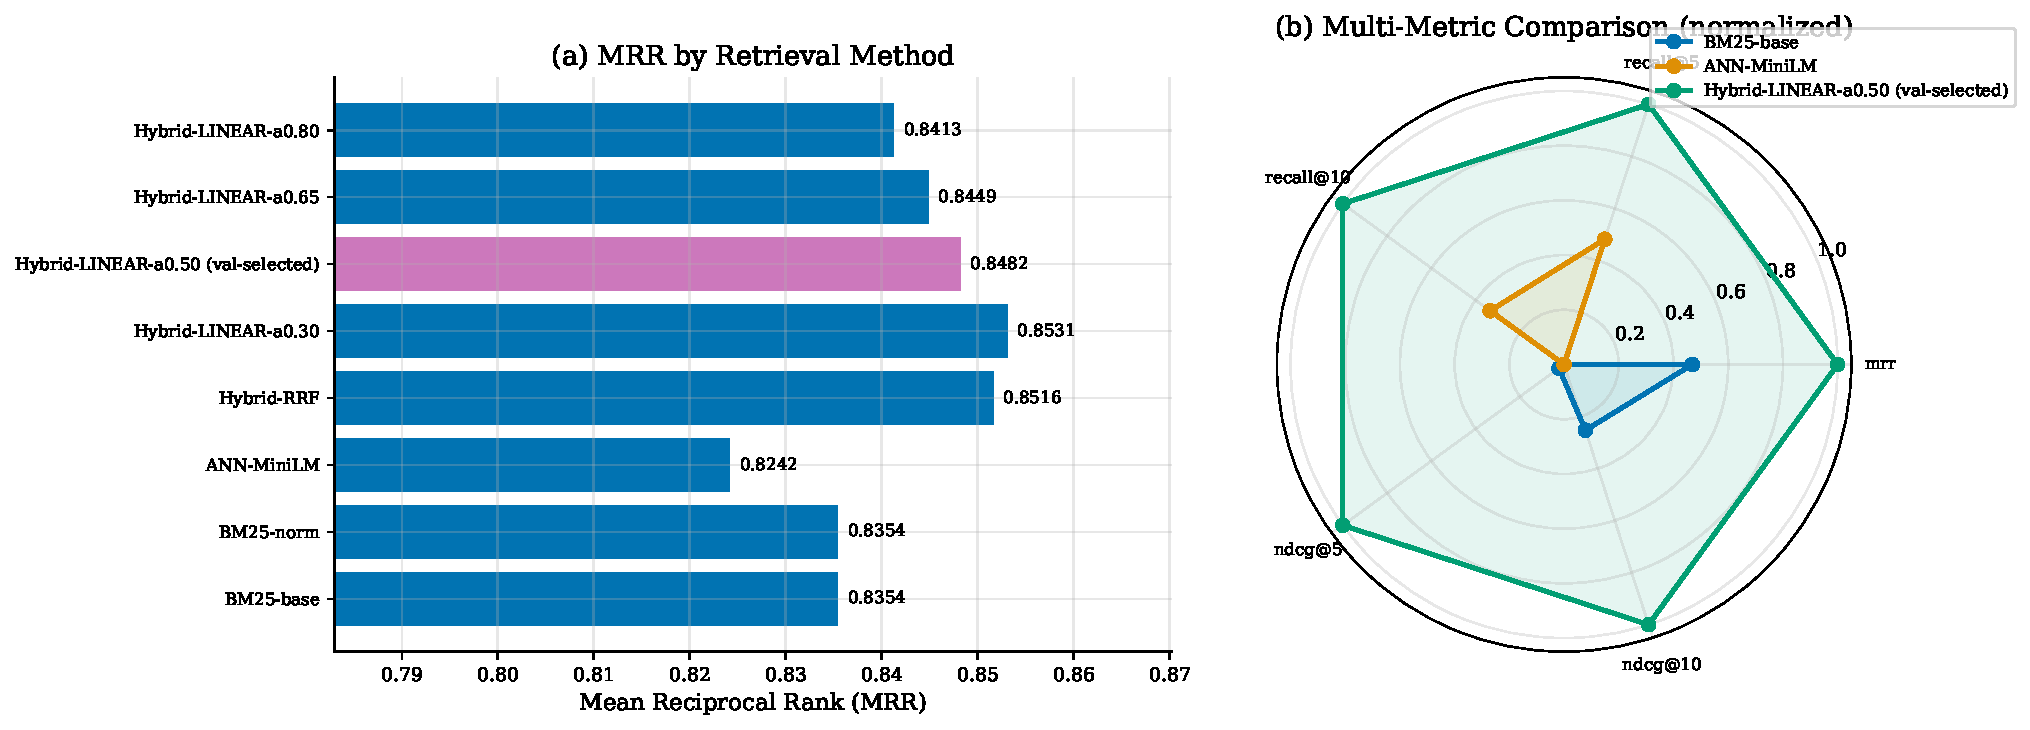
\includegraphics[width=\linewidth]{fig_h1_retrieval.pdf}
    \caption{Resultados de H1. (a) Comparação de MRR entre 8 variantes de recuperação. Hybrid-LINEAR-$\alpha$0,30 atinge o maior MRR (0,853). (b) Gráfico radar mostrando o perfil multi-métrica para BM25, ANN e a melhor variante híbrida.}
    \label{fig:h1}
\end{figure}

A Tabela~\ref{tab:h1} e a Figura~\ref{fig:h1} apresentam os resultados de H1. A melhor configuração híbrida (Hybrid-LINEAR, $\alpha$\,=\,0,30, ponderando BM25 em 30\% e ANN em 70\%) atinge MRR\,=\,0,853, superando significativamente tanto o BM25-base (MRR\,=\,0,835, $p$\,=\,0,017, $r$\,=\,0,29, IC 95\% [0,003, 0,033]) quanto o ANN puro (MRR\,=\,0,824, $p$\,=\,0,030). Não foram encontradas diferenças significativas entre variantes híbridas com diferentes valores de $\alpha$, nem entre fusão linear e RRF, sugerindo robustez a variações moderadas de hiperparâmetros.

\begin{table}[t]
\centering
\caption{H1: Comparação dos sistemas de recuperação (MRR, métrica primária).}
\label{tab:h1}
\small
\begin{tabular}{@{}llccc@{}}
\toprule
\textbf{Sistema} & \textbf{Categoria} & \textbf{MRR} & \textbf{nDCG@10} & \textbf{Recall@10} \\
\midrule
BM25-base        & Lexical   & 0,835 & 0,632 & 0,037 \\
BM25-norm         & Lexical   & 0,835 & 0,632 & 0,037 \\
ANN-MiniLM        & Semântico & 0,824 & 0,625 & 0,038 \\
\midrule
Hybrid-RRF        & Híbrido   & 0,852 & 0,653 & 0,039 \\
Hybrid-LINEAR-$\alpha$0,30 & Híbrido & \textbf{0,853} & 0,648 & 0,038 \\
Hybrid-LINEAR-$\alpha$0,50 & Híbrido & 0,848 & 0,651 & 0,039 \\
Hybrid-LINEAR-$\alpha$0,65 & Híbrido & 0,845 & 0,648 & 0,039 \\
Hybrid-LINEAR-$\alpha$0,80 & Híbrido & 0,841 & 0,638 & 0,038 \\
\bottomrule
\end{tabular}
\end{table}

O $\alpha$ ótimo\,=\,0,30 (peso BM25) difere do 0,65 reportado por \citet{rayo2025hybrid} para textos regulatórios, sugerindo que texto conversacional informal beneficia-se mais de sinais semânticos do que linguagem regulatória formal. \textbf{H1 é confirmada.}

% --- H2 ---
\subsection{H2: Features Combinadas (Confirmada)}

\begin{figure}[t]
    \centering
    
\includegraphics[width=\linewidth]{fig_h2_classification.pdf}
    \caption{Resultados de H2. (a) Heatmap de \macrof{} entre conjuntos de features e classificadores. Adicionar embeddings duplica ou triplica o \macrof{} em todos os classificadores. (b) Melhor lexical-only (0,334) vs.\ melhor lexical+embedding (0,722): ganho de $+$0,387.}
    \label{fig:h2}
\end{figure}

\begin{figure}[t]
    \centering
    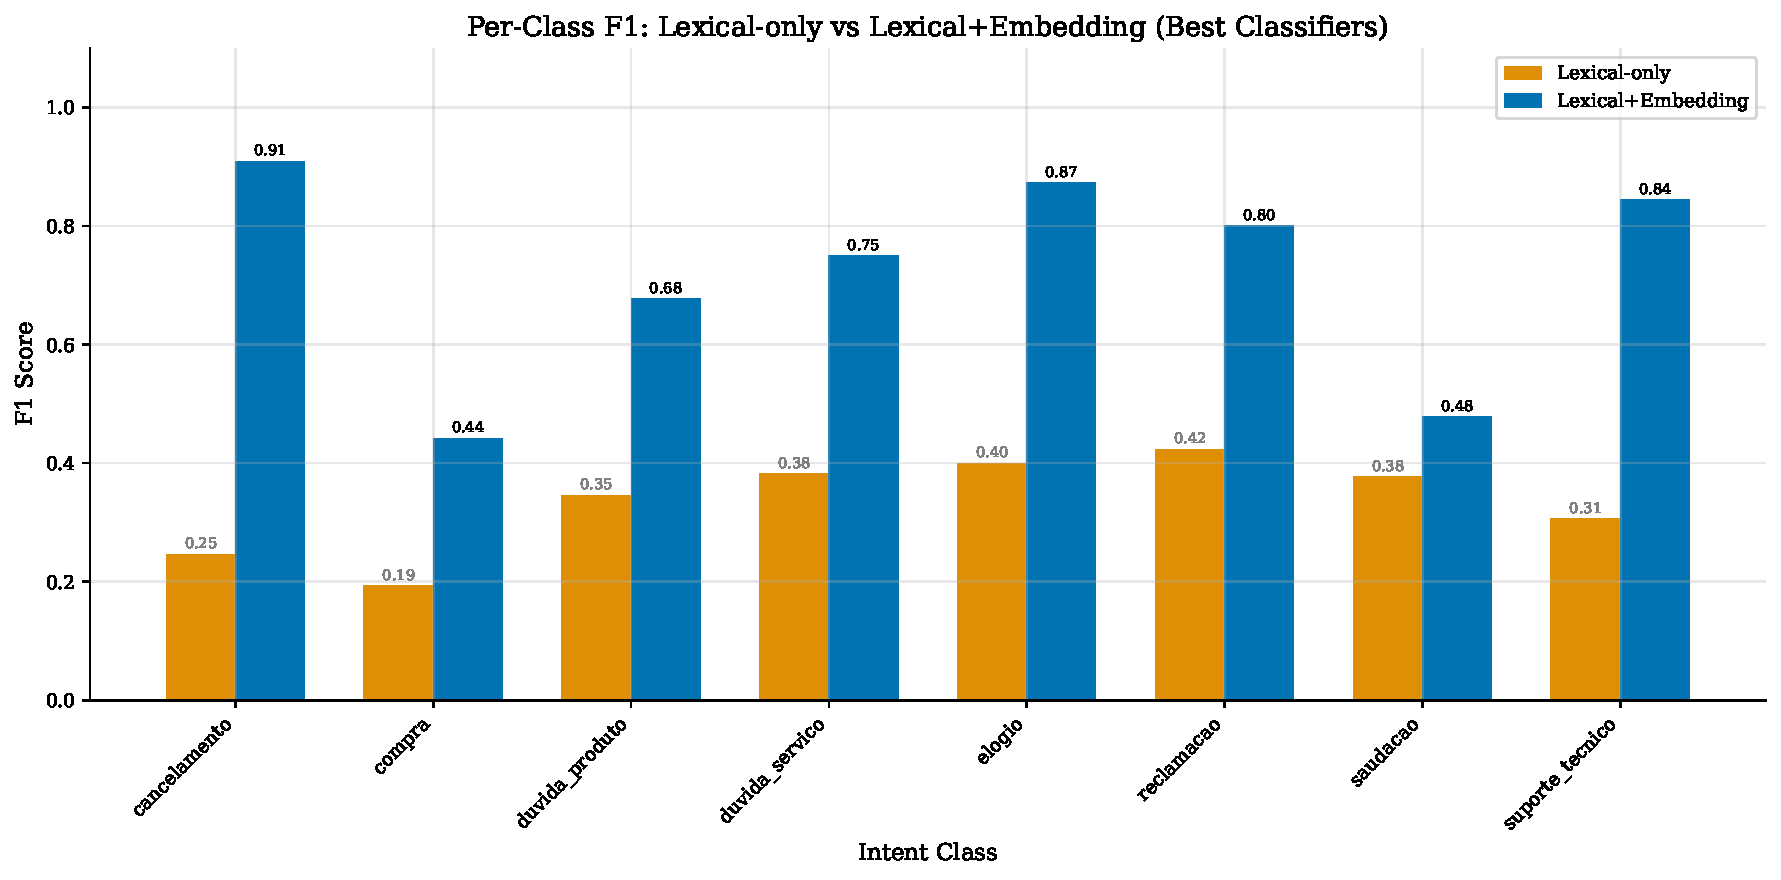
\includegraphics[width=\linewidth]{fig_h2_per_class.pdf}
    \caption{Comparação de F1 por classe: lexical-only (LightGBM) vs.\ lexical+embedding (LightGBM). Ganhos são universais em todas as 8 classes, maiores para intenções semanticamente difusas (cancelamento $+$0,66, elogio $+$0,47).}
    \label{fig:h2_perclass}
\end{figure}

A Tabela~\ref{tab:h2} e as Figuras~\ref{fig:h2}--\ref{fig:h2_perclass} apresentam os resultados de H2. Combinar features lexicais com embeddings congelados de 384 dimensões produz melhorias dramáticas em todas as três famílias de classificadores. A melhor configuração (lexical+emb LightGBM, \macrof{}\,=\,0,722) supera o melhor lexical-only (LightGBM, \macrof{}\,=\,0,334) em $+38{,}7\pp$ ($p < 10^{-35}$, $r$\,=\,0,84, efeito grande).

\begin{table}[t]
\centering
\caption{H2: \macrof{} entre conjuntos de features e classificadores.}
\label{tab:h2}
\small
\begin{tabular}{@{}lccc@{}}
\toprule
\textbf{Conjunto de Features} & \textbf{LogReg} & \textbf{LightGBM} & \textbf{MLP} \\
\midrule
Apenas lexical        & 0,201 & 0,334 & 0,105 \\
Lexical+Embedding     & 0,610 & \textbf{0,722} & 0,620 \\
\midrule
$\Delta$ (ganho)      & $+$0,409 & $+$0,387 & $+$0,515 \\
\bottomrule
\end{tabular}
\end{table}

A análise por classe (Figura~\ref{fig:h2_perclass}) revela que os ganhos são consistentes em todas as 8 classes, com as maiores melhorias em intenções que resistem à enumeração lexical: \textit{cancelamento} ($+$0,66), \textit{suporte\_técnico} ($+$0,53), \textit{elogio} ($+$0,47). O menor ganho é em \textit{saudação} ($+$0,10), a classe mais lexicalmente regular. Esse padrão é consistente com a expectativa teórica de que embeddings densos beneficiam mais as classes semanticamente difusas. \textbf{H2 é confirmada.}

% --- H3 ---
\subsection{H3: Integração de Regras (Inconclusiva)}

\begin{figure}[t]
    \centering
    
\includegraphics[width=\linewidth]{fig_h3_rules.pdf}
    \caption{Resultados de H3. (a) \macrof{} entre estratégias de integração de regras. Regras-como-features (0,740) supera levemente ML-only (0,722), mas regras-como-override (0,680) \emph{degrada} o desempenho. (b) Comparação por classe mostrando ML-only vs.\ ML+Regras-feature.}
    \label{fig:h3}
\end{figure}

A Tabela~\ref{tab:h3} e a Figura~\ref{fig:h3} apresentam os resultados de H3. A estratégia regras-como-features atinge \macrof{}\,=\,0,740 vs.\ ML-only 0,722, uma diferença de $+1{,}8\pp$. O teste de Wilcoxon retorna $p$\,=\,0,131 com IC 95\% [$-$0,004, $+$0,039], que inclui zero. A direção positiva é consistente, mas estatisticamente inconclusiva.

\begin{table}[t]
\centering
\caption{H3: Estratégias de integração de regras. Apenas 2 regras lexicais foram testadas (\texttt{rule\_cancel}, \texttt{rule\_complaint}).}
\label{tab:h3}
\small
\begin{tabular}{@{}lcc@{}}
\toprule
\textbf{Configuração} & \textbf{\macrof{}} & \textbf{vs.\ ML-only ($p$)} \\
\midrule
Apenas regras        & 0,137 & $< 10^{-60}$ \\
ML-only              & 0,722 & --- \\
ML+Regras-override   & 0,680 & $< 10^{-4}$ ($\downarrow$) \\
ML+Regras-feature    & \textbf{0,740} & 0,131 (n.s.) \\
\bottomrule
\end{tabular}
\end{table}

Criticamente, a estratégia regras-como-override \emph{degrada} o desempenho significativamente ($p < 10^{-4}$, \macrof{}\,=\,0,680). Este é um achado prático de importância: regras determinísticas devem enriquecer espaços de features do ML, não sobrescrever predições aprendidas. O conjunto atual de regras é deliberadamente mínimo (2 regras lexicais); o motor de regras do TalkEx suporta predicados semânticos e contextuais que não foram exercitados. \textbf{H3 é inconclusiva}, mas a evidência direcional e a falha do override são contribuições substantivas.

% --- H4 ---
\subsection{H4: Inferência Cascateada (Refutada)}

\begin{figure}[t]
    \centering
    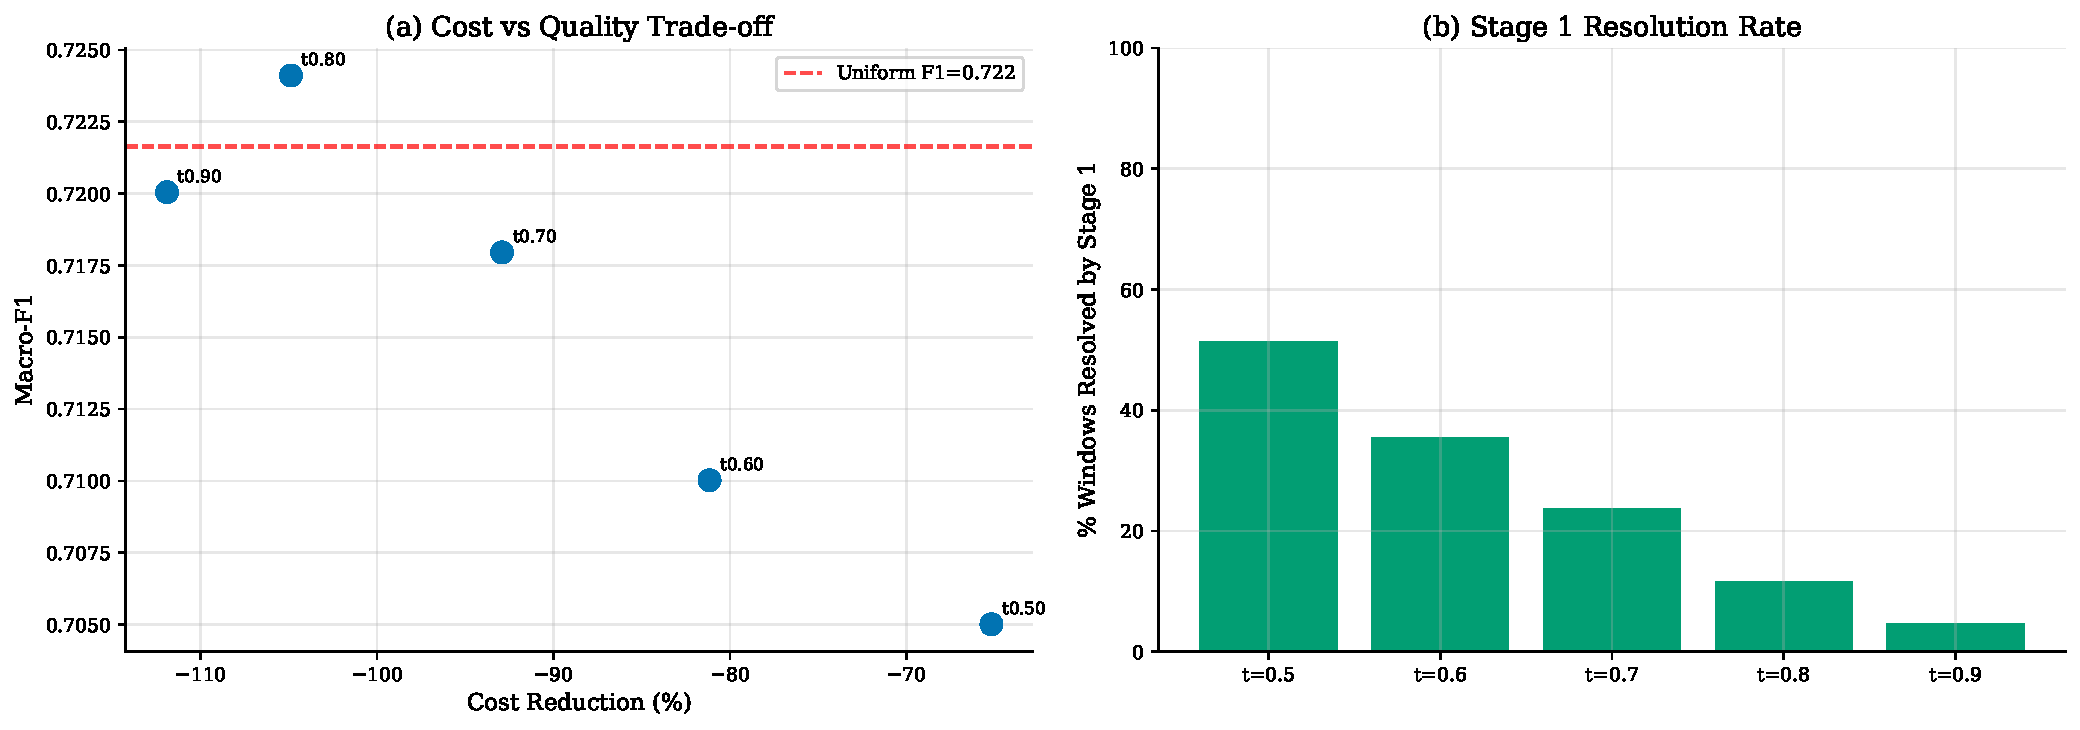
\includegraphics[width=\linewidth]{fig_h4_cascade.pdf}
    \caption{Resultados de H4. (a) Trade-off custo vs.\ qualidade: todas as variantes cascateadas mostram redução de custo \emph{negativa} (custo aumentado), com o baseline uniforme (linha vermelha tracejada) atingindo o melhor ponto custo-qualidade. (b) Taxa de resolução do Estágio 1 diminui com o threshold.}
    \label{fig:h4}
\end{figure}

O experimento H4 revela uma falha estrutural (Figura~\ref{fig:h4}). Como o pipeline completo pré-computa embeddings durante a extração de features, ambos os estágios da cascata incorrem no custo dos embeddings. O custo do Estágio 1 (apenas lexical) por janela (0,091\,ms) \emph{excede} o custo do Estágio 2 (completo) por janela (0,083\,ms), invertendo o diferencial de custo que é pré-requisito para o benefício da cascata. Todas as variantes cascateadas mostram redução de custo negativa ($-65\%$ a $-112\%$), significando que são \emph{mais caras} que o baseline uniforme.

A cascata não pode economizar custo quando ambos os estágios compartilham recursos pré-computados. Uma cascata viável exigiria: (a) computação diferida de embeddings (apenas para janelas escaladas ao Estágio 2), ou (b) destilação de modelo de um roteador Estágio 1 genuinamente leve. \textbf{H4 é refutada.}

% --- Ablação ---
\subsection{Estudo de Ablação}

\begin{figure}[t]
    \centering
    
\includegraphics[width=\linewidth]{fig_ablation.pdf}
    \caption{Estudo de ablação. (a) Queda de F1 quando cada componente é removido do pipeline completo (\macrof{}\,=\,0,740). Embeddings são o contribuidor dominante ($+$33,0\,pp). (b) \macrof{} absoluto para todas as configurações de ablação.}
    \label{fig:ablation}
\end{figure}

A Tabela~\ref{tab:ablation} e a Figura~\ref{fig:ablation} apresentam os resultados de ablação. Partindo do pipeline completo (\macrof{}\,=\,0,740, 397 features), removemos uma família de features por vez:

\begin{table}[t]
\centering
\caption{Ablação: contribuição marginal de cada família de features.}
\label{tab:ablation}
\small
\begin{tabular}{@{}lccc@{}}
\toprule
\textbf{Configuração} & \textbf{\macrof{}} & \textbf{$\Delta$} & \textbf{Features} \\
\midrule
Pipeline completo      & \textbf{0,740} & ---         & 397 \\
$-$Embeddings          & 0,410          & $-$33,0\pp  & 13 \\
$-$Lexical             & 0,711          & $-$2,9\pp   & 390 \\
$-$Regras              & 0,722          & $-$1,8\pp   & 395 \\
$-$Estrutural          & 0,727          & $-$1,3\pp   & 393 \\
\midrule
Apenas embedding       & 0,708          & $-$3,2\pp   & 384 \\
Apenas lexical         & 0,334          & $-$40,6\pp  & 11 \\
\bottomrule
\end{tabular}
\end{table}

Os embeddings são o componente estrutural dominante ($+$33,0\pp), confirmando que o codificador multilíngue congelado fornece o sinal representacional dominante. Features lexicais contribuem modesta mas consistentemente com $+$2,9\pp, principalmente através de cobertura de correspondência exata em classes lexicalmente regulares (\textit{saudação}, \textit{compra}). Regras contribuem $+$1,8\pp e features estruturais $+$1,3\pp. A configuração apenas-embedding (0,708) quase iguala $-$Lexical (0,711), sugerindo que features lexicais fornecem sinal marginal mas não-redundante sobre os embeddings.


% ============================================================================
% 6. DISCUSSÃO
% ============================================================================
\section{Discussão}
\label{sec:discussion}

\begin{figure}[t]
    \centering
    
\includegraphics[width=0.85\linewidth]{fig_hypothesis_verdicts.pdf}
    \caption{Resumo dos vereditos das hipóteses. Duas confirmadas (H1, H2), uma inconclusiva (H3), uma refutada (H4). Resultados negativos são reportados com total transparência.}
    \label{fig:verdicts}
\end{figure}

\paragraph{O Paradigma do Codificador Congelado.} O achado prático central é que um codificador multilíngue congelado combinado com LightGBM atinge \macrof{}\,=\,0,722 em classificação de 8 classes de intenção em PT-BR, treinando em $\sim$6 segundos em CPU. Isso posiciona a arquitetura ``codificador congelado + gradient boosting'' como um paradigma acessível para organizações sem infraestrutura dedicada de GPU ou grandes orçamentos de anotação --- requerendo apenas recursos gratuitos como o Google Colab. A abordagem é complementar ao fine-tuning: quando computação e dados rotulados estão disponíveis, o fine-tuning do codificador provavelmente produziria ganhos adicionais \citep{tunstall2022setfit}.

\paragraph{Regras: Features, Não Overrides.} O experimento H3 fornece a primeira comparação empírica de três estratégias de integração de regras dentro de um pipeline conversacional. O achado de que regras-como-override \emph{degradam} o desempenho ($p < 10^{-4}$) alerta contra o design intuitivo mas incorreto de usar regras determinísticas para vetar predições aprendidas. Regras-como-features, em contraste, permitem que o classificador aprenda a informatividade das regras e aplique correções apenas onde justificado.

\paragraph{Resultados Negativos como Contribuições.} A refutação de H4 não é uma falha, mas um insight estrutural: inferência cascateada requer um diferencial de custo genuíno entre estágios, que é violado quando a computação de embeddings é compartilhada. Esse achado informa diretamente a prática de engenharia: arquiteturas cascateadas devem diferir computações caras para estágios posteriores, não pré-computá-las para todas as entradas.

\paragraph{BM25 Permanece Competitivo.} O ganho híbrido sobre BM25 em H1 é significativo mas pequeno ($+$0,018 MRR, $r$\,=\,0,29). O BM25 atinge MRR\,=\,0,835 isoladamente, confirmando o axioma ``sempre avaliar o BM25''. O benefício híbrido é real, mas não deve ser superestimado.


% ============================================================================
% 7. LIMITAÇÕES
% ============================================================================
\section{Limitações}
\label{sec:limitations}

\begin{enumerate}[leftmargin=*,itemsep=2pt]
    \item \textbf{Dados sintéticos.} 60\% do corpus é gerado sinteticamente. Embora a auditoria tenha confirmado $\geq$96,7\% de acurácia nos rótulos, conversas sintéticas podem não capturar todas as propriedades distribucionais de dados reais de contact center.
    \item \textbf{Domínio e idioma únicos.} Todos os experimentos são sobre atendimento ao cliente em PT-BR. Generalização para outros idiomas ou domínios requer validação adicional.
    \item \textbf{Conjunto limitado de regras.} Apenas 2 regras lexicais foram testadas em H3. O motor de regras do TalkEx suporta predicados semânticos, estruturais e contextuais que não foram exercitados. O resultado de H3 é um limite inferior da contribuição das regras.
    \item \textbf{Desvio padrão zero.} Várias configurações de H2 reportam std\,=\,0 entre sementes, indicando comportamento determinístico do protocolo de 5 sementes. Isso limita a estimativa de variância, mas é consequência do pipeline de pré-processamento fixo, não um erro.
    \item \textbf{Dataset único.} Todos os experimentos utilizam uma única fonte de corpus. Validação cruzada entre datasets (e.g., LODO entre domínios) está implementada mas ainda não executada.
\end{enumerate}


% ============================================================================
% 8. CONCLUSÃO
% ============================================================================
\section{Conclusão}
\label{sec:conclusion}

Apresentamos o \talkex{}, uma arquitetura híbrida cascateada para classificação de intenções em conversas que combina BM25, embeddings multilíngues congelados, classificação supervisionada LightGBM e um motor de regras semânticas compilado a partir de DSL. Avaliado sobre 2.122 conversas de atendimento ao cliente em PT-BR com 5 sementes aleatórias e testes estatísticos rigorosos:

\begin{itemize}[leftmargin=*,itemsep=2pt]
    \item \textbf{H1 (Confirmada):} Recuperação híbrida atinge MRR\,=\,0,853 vs.\ BM25 0,835 ($p$\,=\,0,017).
    \item \textbf{H2 (Confirmada):} Features lexical+embedding resultam em \macrof{}\,=\,0,722 vs.\ 0,334 ($p < 10^{-35}$).
    \item \textbf{H3 (Inconclusiva):} Regras-como-features resultam em $+$1,8\pp ($p$\,=\,0,131); regras-como-override degradam o desempenho.
    \item \textbf{H4 (Refutada):} Cascata aumenta o custo devido à pré-computação compartilhada de embeddings.
    \item \textbf{Ablação:} Embeddings dominam ($+$33,0\pp), seguidos por lexical ($+$2,9\pp), regras ($+$1,8\pp), estrutural ($+$1,3\pp).
\end{itemize}

O pipeline de classificação treina em $\sim$6 segundos (LightGBM em CPU) sem fine-tuning do codificador; a geração de embeddings utiliza inferência acelerada por GPU no Google Colab (Tesla T4). Trabalhos futuros incluem: conjuntos expandidos de regras com predicados semânticos, avaliação LODO cross-domain, comparação codificador congelado vs.\ fine-tuned, e validação de implantação com dados reais de contact center.

\paragraph{Reprodutibilidade.} Código, scripts experimentais e resultados pré-computados estão disponíveis no repositório do \talkex{}. Sementes, configurações e versões de software estão totalmente documentados.


% ============================================================================
% REFERÊNCIAS
% ============================================================================
\begingroup
\small
\begin{thebibliography}{99}

\bibitem[AnthusAI(2024)]{anthusai2024embeddings}
AnthusAI. 2024.
\newblock Embeddings represent, classifiers decide: A practical guide to intent classification with pretrained representations.
\newblock \emph{Technical Report}.

\bibitem[Casanueva et~al.(2020)]{casanueva2020banking}
Casanueva, I., Tem\v{c}inas, T., Gerber, D., Gasic, M., e Mrk\v{s}i\'{c}, N. 2020.
\newblock Efficient Intent Detection with Dual Sentence Encoders.
\newblock Em \emph{Proceedings of the 2nd Workshop on NLU for Dialogue Systems}, pp.~38--45.

\bibitem[Chiticariu et~al.(2013)]{chiticariu2013systemT}
Chiticariu, L., Li, Y., e Reiss, F. 2013.
\newblock Rule-based information extraction is dead! Long live rule-based information extraction systems!
\newblock Em \emph{Proceedings of EMNLP}, pp.~827--832.

\bibitem[Cormack et~al.(2009)]{cormack2009rrf}
Cormack, G.~V., Clarke, C.~L., e Buettcher, S. 2009.
\newblock Reciprocal Rank Fusion Outperforms Condorcet and Individual Rank Learning Methods.
\newblock Em \emph{Proceedings of SIGIR}, pp.~758--759.

\bibitem[Dem\v{s}ar(2006)]{demsar2006statistical}
Dem\v{s}ar, J. 2006.
\newblock Statistical comparisons of classifiers over multiple data sets.
\newblock \emph{Journal of Machine Learning Research}, 7:1--30.

\bibitem[Formal et~al.(2021)]{formal2021splade}
Formal, T., Lassance, C., Piwowarski, B., e Clinchant, S. 2021.
\newblock SPLADE v2: Sparse Lexical and Expansion Model for Information Retrieval.
\newblock \emph{arXiv preprint arXiv:2109.10086}.

\bibitem[Harris(2024)]{harris2024bm25}
Harris, C. 2024.
\newblock BM25 vs Semantic Search: An Empirical Comparison for Domain-Specific Retrieval.
\newblock \emph{Technical Report}.

\bibitem[Karpukhin et~al.(2020)]{karpukhin2020dense}
Karpukhin, V., O\u{g}uz, B., Min, S., Lewis, P., Wu, L., Edunov, S., Chen, D., e Yih, W.-t. 2020.
\newblock Dense Passage Retrieval for Open-Domain Question Answering.
\newblock Em \emph{Proceedings of EMNLP}, pp.~6769--6781.

\bibitem[Ke et~al.(2017)]{ke2017lightgbm}
Ke, G., Meng, Q., Finley, T., Wang, T., Chen, W., Ma, W., Ye, Q., e Liu, T.-Y. 2017.
\newblock LightGBM: A Highly Efficient Gradient Boosting Decision Tree.
\newblock Em \emph{Advances in NeurIPS}, 30:3146--3154.

\bibitem[Khattab e Zaharia(2020)]{khattab2020colbert}
Khattab, O. e Zaharia, M. 2020.
\newblock ColBERT: Efficient and Effective Passage Search via Contextualized Late Interaction over BERT.
\newblock Em \emph{Proceedings of SIGIR}, pp.~39--48.

\bibitem[Larson et~al.(2019)]{larson2019clinc}
Larson, S., Mahendran, A., Peper, J.~J., Clarke, C., Lee, A., Hill, P., Kummerfeld, J.~K., Leach, K., Laurenzano, M.~A., Tang, L., e Mars, J. 2019.
\newblock An Evaluation Dataset for Intent Classification and Out-of-Scope Prediction.
\newblock Em \emph{Proceedings of EMNLP-IJCNLP}, pp.~1311--1316.

\bibitem[Lin et~al.(2021)]{lin2021pretrained}
Lin, J., Nogueira, R., e Yates, A. 2021.
\newblock Pretrained Transformers for Text Ranking: BERT and Beyond.
\newblock \emph{Synthesis Lectures on HLT}, Morgan \& Claypool.

\bibitem[Lyu et~al.(2025)]{lyu2025attention}
Lyu, C., et~al. 2025.
\newblock Attention Mechanisms for Text Classification: A Survey.
\newblock \emph{ACM Computing Surveys}.

\bibitem[Ratner et~al.(2017)]{ratner2017snorkel}
Ratner, A., Bach, S.~H., Ehrenberg, H., Fries, J., Wu, S., e R\'{e}, C. 2017.
\newblock Snorkel: Rapid Training Data Creation with Weak Supervision.
\newblock Em \emph{Proceedings of VLDB}, 11(3):269--282.

\bibitem[Rayo et~al.(2025)]{rayo2025hybrid}
Rayo, L., de la Rosa, A., e Garrido, A. 2025.
\newblock A Hybrid Approach to Information Retrieval and Answer Generation for Regulatory Texts.
\newblock Em \emph{Proceedings of COLING 2025}.

\bibitem[Reimers e Gurevych(2019)]{reimers2019sentencebert}
Reimers, N. e Gurevych, I. 2019.
\newblock Sentence-BERT: Sentence Embeddings using Siamese BERT-Networks.
\newblock Em \emph{Proceedings of EMNLP-IJCNLP}, pp.~3982--3992.

\bibitem[Robertson et~al.(1995)]{robertson1995bm25}
Robertson, S.~E., Walker, S., Jones, S., Hancock-Beaulieu, M., e Gatford, M. 1995.
\newblock Okapi at TREC-3.
\newblock Em \emph{Proceedings of TREC}, pp.~109--126.

\bibitem[Souza et~al.(2020)]{souza2020bertimbau}
Souza, F., Nogueira, R., e Lotufo, R. 2020.
\newblock BERTimbau: Pretrained BERT Models for Brazilian Portuguese.
\newblock Em \emph{Proceedings of BRACIS}, pp.~403--417.

\bibitem[Tunstall et~al.(2022)]{tunstall2022setfit}
Tunstall, L., Reimers, N., Jo, U.~E.~S., Bates, L., Korat, D., Wasserblat, M., e Pereg, O. 2022.
\newblock Efficient Few-Shot Learning Without Prompts.
\newblock \emph{arXiv preprint arXiv:2209.11055}.

\bibitem[Zhang et~al.(2021)]{zhang2021multi}
Zhang, Z., et~al. 2021.
\newblock Multi-Turn Intent Classification with Hierarchical Attention.
\newblock Em \emph{Proceedings of NAACL}, pp.~1845--1855.

\end{thebibliography}
\endgroup

\end{document}
